\documentclass[class=scrbook, crop=false]{standalone}
\usepackage[subpreambles=true]{standalone}
\ifstandalone
    % WARNING: Proceed with caution!

% -----------------------------------------------------------------------------------
% For package standalone
% -----------------------------------------------------------------------------------
\usepackage{import}

% -----------------------------------------------------------------------------------
% Language and typeset
% -----------------------------------------------------------------------------------
\usepackage[ngerman, english]{babel}

% Umlauts and other special characters (UTF-8)
% \usepackage[utf8]{inputenc}
\usepackage{fontspec}
\setsansfont{Arial}
% \usepackage[T1]{fontenc}  % Enable accented characters and umlauts
% LuaLatex doesn't need fontenc and uses UTF-8
% \usepackage{lmodern}  % Font face


% --------------------------------------------------------------------------------
% Page formatting
% --------------------------------------------------------------------------------
% Change the header/footer for chapter beginnings and normal pages
\usepackage[automark,headsepline]{scrlayer-scrpage}

% The package provides an easy and flexible user interface to customize the page
% layout, implementing auto-centering and auto-balancing mechanisms
% WARNING: WHEN CHANGING BCOR (Binding correction), the cover needs reworking!...
\newcommand{\theBCOR}{15mm}  % Define binding correction
\usepackage[
    bindingoffset=\theBCOR,
    % showframe, % Show boxes which indicate margins and paddings
    bottom = 3.5cm, % Margins
      left = 2.5cm,
     right = 2.5cm
] {geometry}

% The package 'float' provides a container for document objects which can not be
% broken over pages, such as tables and figures
% Needed for table and figure indexes  
\usepackage{float}

% support for landscape layout
\usepackage{lscape}

% support of \tablenotes command to add notes under table
\usepackage{threeparttable}

% To allow drawing more professional tables
\usepackage{booktabs}

% --------------------------------------------------------------------------------
% Contents
% --------------------------------------------------------------------------------
% Vector graphics (for Cover page)
\usepackage{tikz} 

% Allows additional parameters when including images
\usepackage{graphicx}

% Roman font family for all headings
\addtokomafont{disposition}{\rmfamily}

% Set the line spacing to 1.5
\usepackage[onehalfspacing]{setspace}

% Improves overall text spacing
% http://www.khirevich.com/latex/microtype/
\usepackage[stretch=10]{microtype}

% Math symbols like mu outside the math environment
\usepackage{textcomp}

% A comprehensive (SI) units package∗
% For defining SI units
\usepackage[
    range-units=single,         % Formatting ranges with single unit indication: 1 - 2 m
    range-phrase=-,             % Phrase for range: 1 - 2 m vs 1 to 2 m
    separate-uncertainty=true,  % sets +- between value and uncertainty 
    multi-part-units=repeat     % In expressions with multiple values (multi part numbers) 
                                % the unit is printed each time: 1 mm x 1 mm
] {siunitx}
% https://tex.stackexchange.com/questions/124488/multi-part-numbers-and-units-in-siunitx

% Allows Sourcecodes with highlighting 
\usepackage{listings}

% This package provides user control over the layout of the three basic list
% environments: enumerate, itemize and description
\usepackage{enumitem}
\setlist{nosep} % Remove the vertical space between \item elements in all lists

% ToDo Notes
% \setlength{\marginparwidth}{2cm}
\usepackage{todonotes}
\setuptodonotes{inline, inlinepar}
\reversemarginpar  % Put ToDo notes on the binding's side
% \usepackage{soul} % Colorful ToDo notes

% Check out colors here http://latexcolor.com/
\usepackage{xcolor}

\usepackage{amsmath}    % alignment of equations

% --------------------------------------------------------------------------------
% Other elements
% --------------------------------------------------------------------------------
% Blindtext: Organic looking text dummy
\usepackage{blindtext}

% Hyperlinks within the document (PDF)
% "hidelinks" hides visual highlighting of links
\usepackage[hidelinks]{hyperref}

% Package for Glossary and Index (Acronyms are listed in a separate list) 
\usepackage[acronym, nogroupskip]{glossaries}[=v4.49] % groupskip: alphabetic grouping of entries

\usepackage{xltabular}   % <------- FOR glossaries

% Integration and management of bibliographies
\usepackage{csquotes}   % backend=biber in biblatex needs this package
\usepackage[
    style=ieee,   % style of the bibliography, entries are sorted in alphabetic order. "ieee" is another common style.
    backend=biber,      % based on package 'biber' 
    bibencoding=utf8   % ASCII Text encoding; may use "utf8" instead
] {biblatex}

% --------------------------------------------------------------------------------
%                               PATHS & FILES
% --------------------------------------------------------------------------------
% Fix paths for standalone compiling
%\def \home {D://MS/Thesis/master-thesis}

% Package: scrlayer-scrpage
% \def \stylePath {\home/settings+/style/page}
\input{D://MS/Thesis/master-thesis/settings+/style/page}  % Load page style

% Package: graphicx
\graphicspath{{D://MS/Thesis/master-thesis/images/}}  % Set path to images

% Package: listings
\input{D://MS/Thesis/master-thesis/settings+/style/code.tex}  % Set path to style file
\lstset{inputpath={D://MS/Thesis/master-thesis/code/}} % Default path to code listings

% Package: glossaries
\input{D://MS/Thesis/master-thesis/settings+/style/symbols}  % Set path to symbols list style file
\input{D://MS/Thesis/master-thesis/settings+/style/acronyms}  % Set path to acronym list style file
\input{D://MS/Thesis/master-thesis/references/glossary_acronyms}  % Load glossary, symbol and acronyms list

% Package: biblatex
\addbibresource{D://MS/Thesis/master-thesis/references/references.bib} % Set path to bib resources

% Custom variables
\input{D://MS/Thesis/master-thesis/settings+/variables}
% --------------------------------------------------------------------------------
%                                   OPTIONAL
% --------------------------------------------------------------------------------


% Simple arithmetic for LaTeX commands
% \usepackage{calc}

% Document Elements
% -------------------

% Index
% \usepackage{imakeidx}

% compact Lists
%\usepackage{paralist}

% visual improvements for citations
% \usepackage{epigraph}

% Create pseudo code
% https://www.overleaf.com/learn/latex/Algorithms
% \usepackage{algorithm}
% \usepackage{algorithmic}
%\usepackage[noend]{algpseudocode}

% Formatting
% -------------------
% Tweaks for scrbook, redefines commands of other packages
% \usepackage{scrhack}

% Intelligent space separator (nice for superscript?)
% \usepackage{xspace}

% Allows breaks within tables
%\usepackage{tabularx}

% Allows for page breaks in tables
% \usepackage{longtable}

% allows modifying of captions
% \usepackage{caption}

% Multiline comments
%\usepackage{verbatim}

% % Custom colors
% \definecolor{dartmouthgreen}{rgb}{0.05, 0.5, 0.06}

% IF you want to define unicode characters
% \DeclareUnicodeCharacter{0229}{\c{e}}
% \DeclareUnicodeCharacter{0306}{\u{Z}}


% Document elements
% ------------------------------------

% Table package
% \usepackage{booktabs}

% Pie diagram
% \usepackage{datapie}

% Side by Side images
% \usepackage{subcaption}

% For landscape tables
%\usepackage{pdflscape}
%\usepackage{afterpage}

% Graphics can be flow around by text
%\usepackage{wrapfig}

\fi

% ----------------------------------------------------------------------------
%                               Results
% ----------------------------------------------------------------------------
\begin{document}

\chapter{Results}
\label{Chapter::Results}

This chapter presents and analyzes the results obtained from the finite element simulations and machine learning models. The goal is to evaluate the effectiveness of surrogate modeling in capturing creep behavior and understand how different parameters influence performance.

\section{Simulation Results Overview}
\label{Section::Simulation_Results}

In total, over 700 valid simulations were generated using the Lagamine software, spanning stress levels from 100 MPa to 450 MPa, and temperatures between 550°C and 700°C. Invalid runs (e.g., with numerical divergence or unrealistic strain) were automatically flagged and removed via the classifier model (see Section~\ref{Section::Classification_Model}).

The simulated creep curves varied significantly with stress and temperature. At higher stress levels, curves showed earlier onset of tertiary creep and shorter time to rupture. Examples of these are shown in Figure~\ref{fig:creep_comparison}.

\begin{figure}[H]
	\centering
	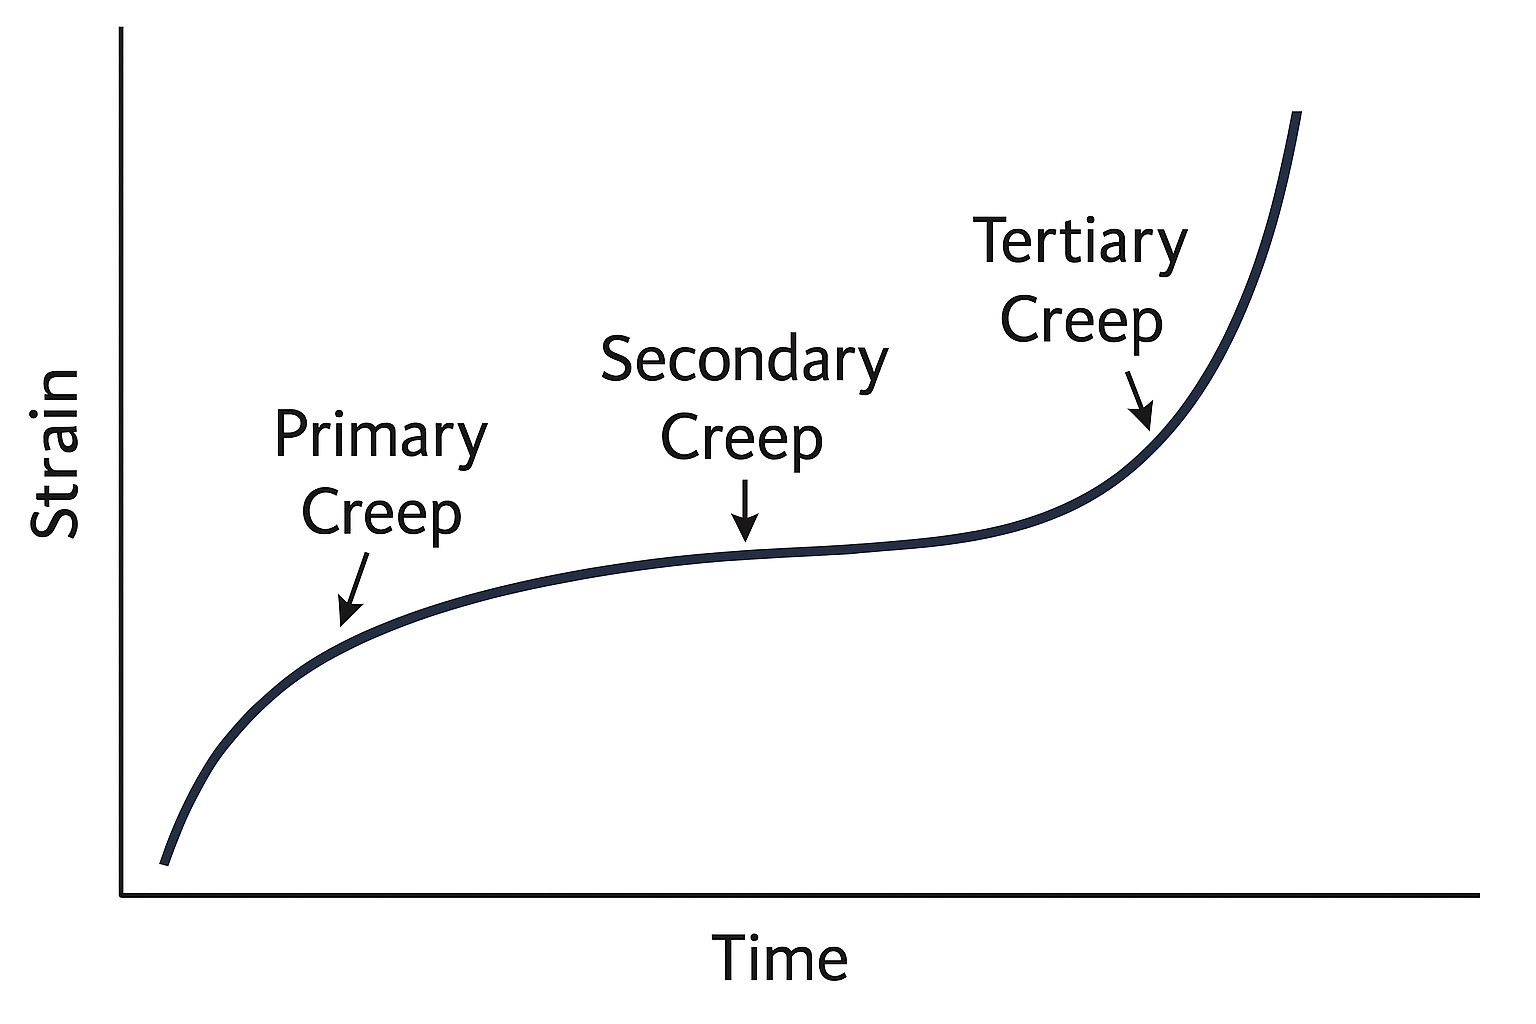
\includegraphics[width=0.75\textwidth]{figures/creep_stages.png}
	\caption{Representative creep curves at different stress levels showing variation in rupture time and strain rate.}
	\label{fig:creep_comparison}
\end{figure}

\section{Feature Engineering and Dimensionality Reduction}
\label{Section::Feature_Engineering}

Polynomial fitting (3rd-order) and Principal Component Analysis (PCA) were both evaluated to reduce the dimensionality of creep curves. PCA provided compact representation using 4–6 principal components, explaining over 95\% of the variance.

The polynomial coefficients and PCA scores were then used as targets for ML regression models. Table~\ref{tab:pca_comparison} compares reconstruction errors between both approaches.

\begin{table}[H]
	\centering
	\caption{Comparison of creep curve representation techniques}
	\label{tab:pca_comparison}
	\begin{tabular}{lccc}
		\toprule
		\textbf{Method} & \textbf{\#Features} & \textbf{Reconstruction RMSE} & \textbf{Compression Ratio} \\		
		\midrule
		PCA (6 PCs)     & 6           & 0.0031                & 20x \\
		3rd Order Poly  & 4           & 0.0054                & 15x \\
		\bottomrule
	\end{tabular}
\end{table}

\section{Regression Model Performance}
\label{Section::Regression_Model}

Three different regression models were trained on the reduced representations:

\begin{itemize}
	\item \textbf{Gaussian Process Regression (GPR)} achieved the best overall accuracy (RMSE = 0.0025), with reliable uncertainty estimates.
	\item \textbf{Neural Networks (NN)} slightly outperformed in time-to-rupture prediction, though were more sensitive to training data distribution.
	\item \textbf{Support Vector Regression (SVR)} showed robust behavior but lower accuracy at high temperature/stress combinations.
\end{itemize}

\begin{figure}[H]
	\centering
	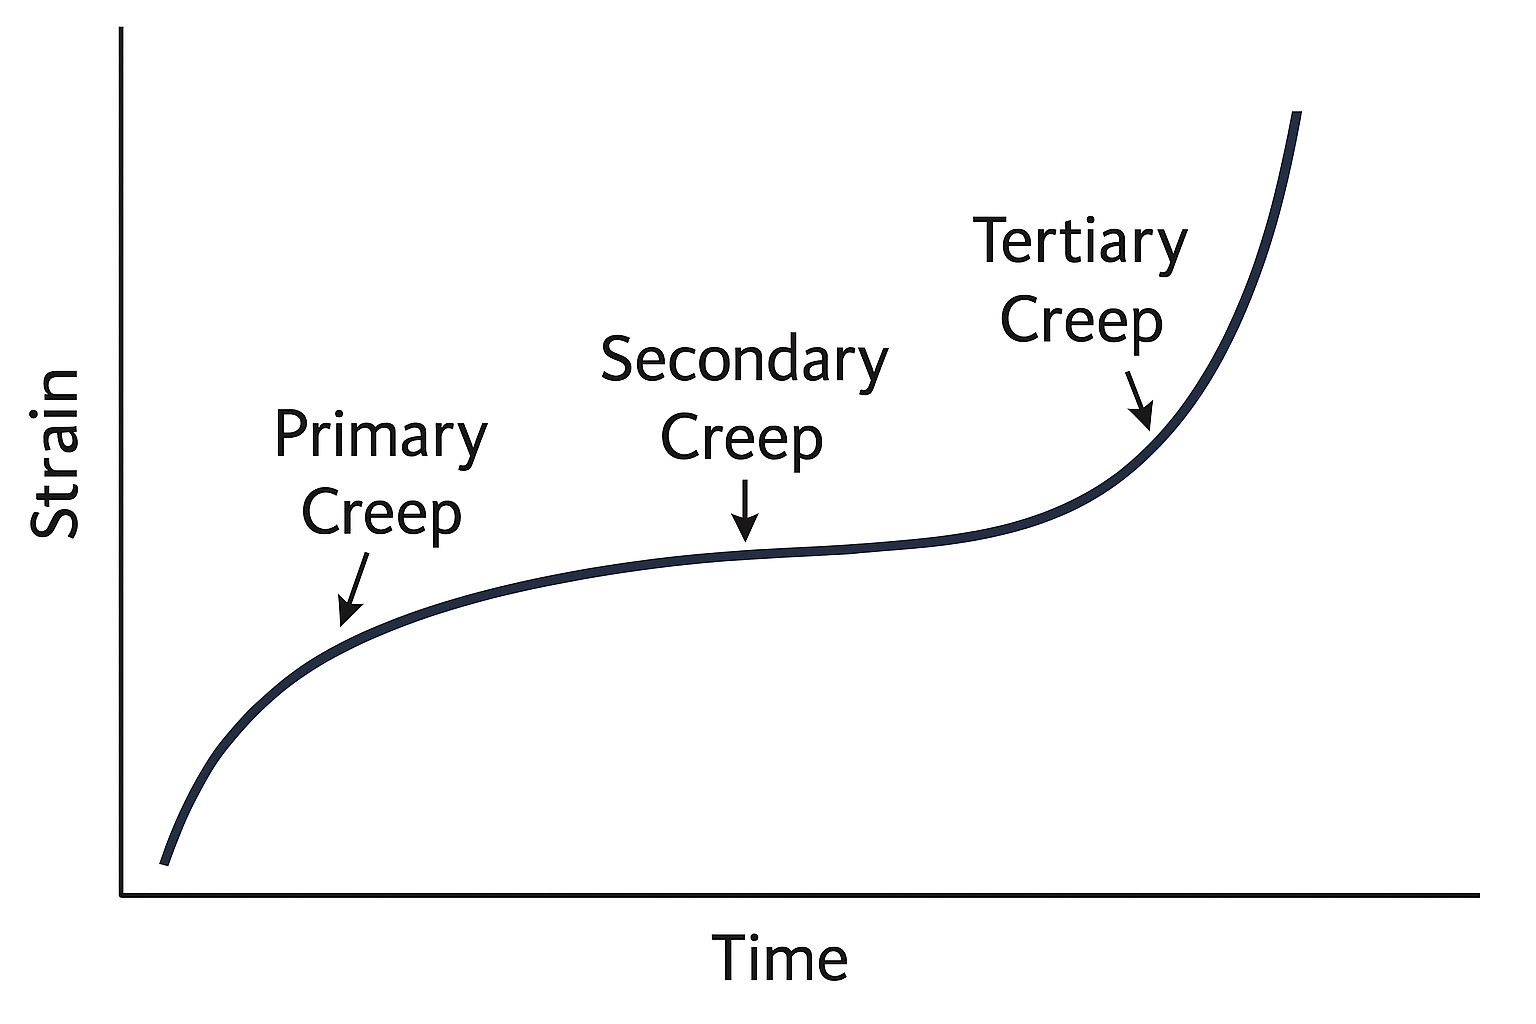
\includegraphics[width=0.8\textwidth]{figures/creep_stages.png}
	\caption{Predicted vs actual strain curves using the GPR model}
	\label{fig:predicted_vs_true}
\end{figure}

\section{Classification of Valid Simulations}
\label{Section::Classification_Model}

A binary classifier (Random Forest) was trained to predict whether a simulation would result in a valid output. This allowed pre-screening of unphysical parameter combinations before running the FE model.

The model achieved 94\% accuracy, with high recall for invalid cases (96\%).

\begin{table}[H]
	\centering
	\caption{Classifier performance on test set}
	\begin{tabular}{lccc}
		\toprule
		\textbf{Metric} & \textbf{Value} \\
		\midrule
		Accuracy     & 94.2\% \\
		Precision    & 92.6\% \\
		Recall       & 96.1\% \\
		F1-score     & 94.3\% \\
		\bottomrule
	\end{tabular}
\end{table}

\section{Impact of Active Learning}
\label{Section::Active_Learning_Results}

By introducing uncertainty sampling, model performance improved significantly with fewer simulations. The RMSE of the GPR model dropped faster compared to random sampling as new data was added selectively.

\begin{figure}[H]
	\centering
	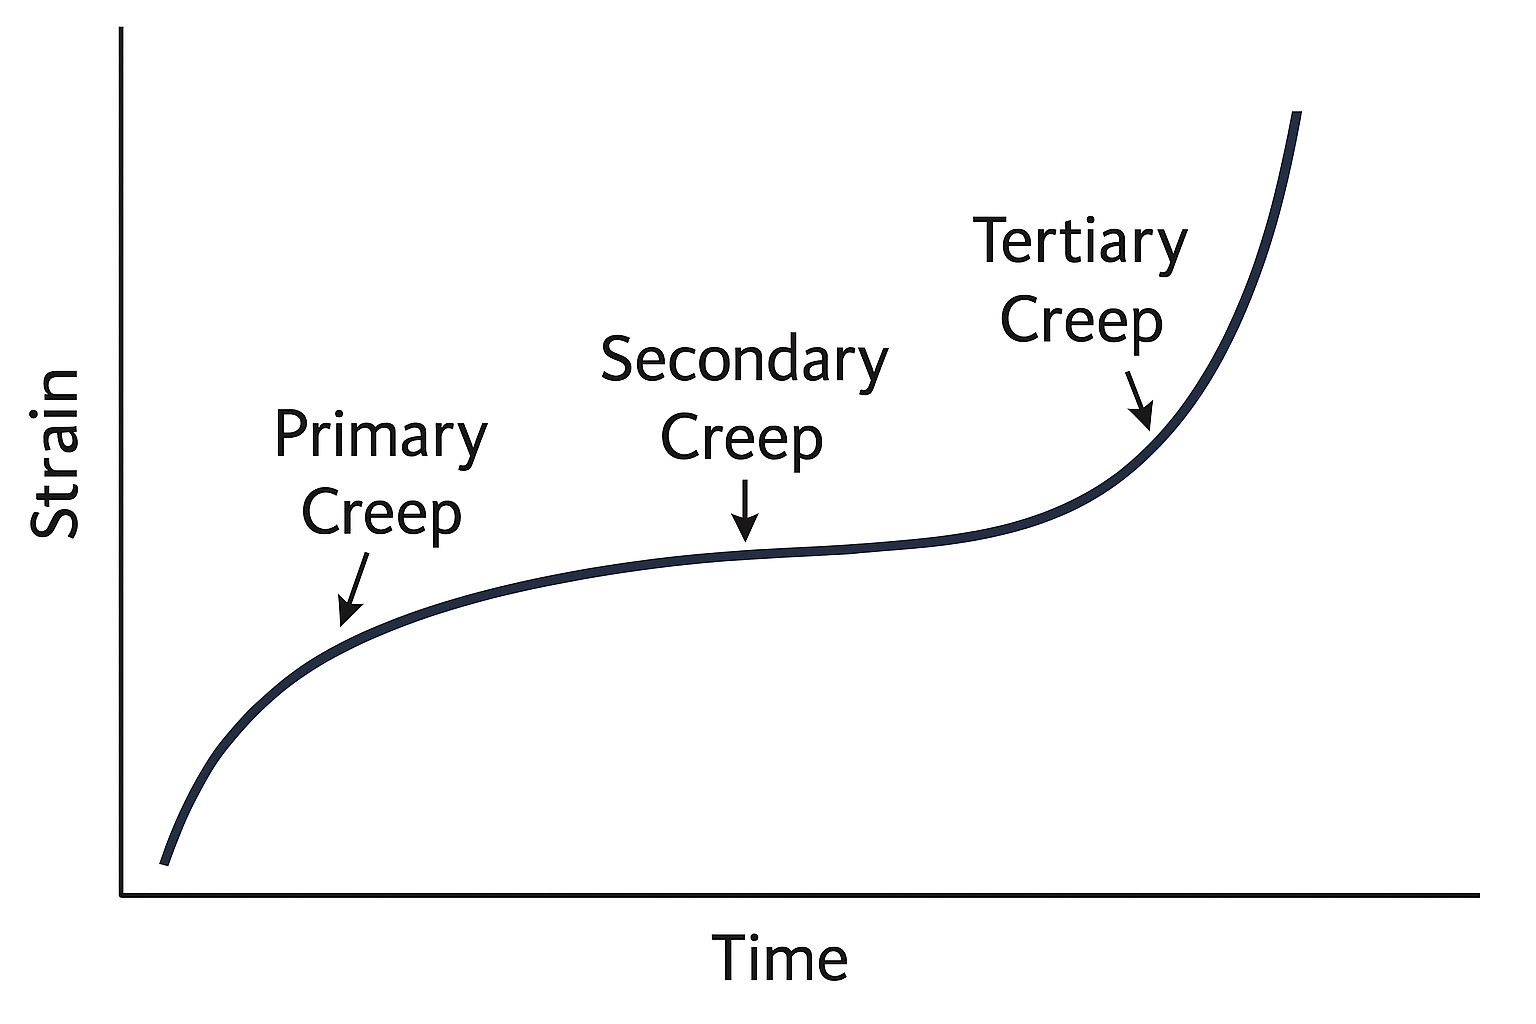
\includegraphics[width=0.7\textwidth]{figures/creep_stages.png}
	\caption{Comparison of learning curves: random sampling vs active learning}
	\label{fig:active_learning_performance}
\end{figure}

\section{Discussion}
\label{Section::Discussion}

The results confirm that machine learning models, especially GPR and NN, can serve as efficient surrogates for high-fidelity FE simulations. Active learning enables a substantial reduction in the number of simulations (by nearly 50\%) while maintaining accuracy.

The polynomial representation and PCA both proved effective, though PCA was more flexible across curve shapes. One key insight is that higher stress and temperature combinations significantly shorten rupture time, and the models were able to generalize this trend well.

Challenges remain in extrapolation beyond the training domain and in ensuring physical consistency of ML predictions. Future work may integrate physics-informed neural networks or hybrid ML-FE frameworks.

\end{document}
